
\documentclass[11pt]{article}
\usepackage[paper=letterpaper, margin=.75in]{geometry}
\linespread{1.5}
\pdfpagewidth 8.5in
\pdfpageheight 11in

%%% Packages
% First four - AMS (american mathematical society). General math goodness. I use the align* enviorment in particular
% multirow, multicol allow for certain kinds of tables
% enumerate lets you determine the style of the counter for the enumerate enviorment
% graphicx lets you include pictures
% listings lets you stick in blocks of code
% placeins defines "\FloatBarrier", which stops tables from moving around
\usepackage{amsmath, amscd, amssymb, amsthm, multirow, multicol, enumerate, graphicx, listings, placeins, caption,hyperref} 
\usepackage[utf8]{inputenc}
\usepackage[english]{babel}
\usepackage[style=numeric,backend=biber]{biblatex}
\addbibresource{bibli.bib}

\captionsetup{font={small,singlespacing},margin=1cm}
\newcommand{\Z}{\mathbb{Z}}
\newcommand{\R}{\mathbb{R}}
\newcommand{\Q}{\mathbb{Q}}
\newcommand{\C}{\mathbb{C}}
\newcommand{\N}{\mathbb{N}}
\newcommand{\V}{\mathbb{V}}
\newcommand{\U}{\mathcal{U}}
\newcommand{\del}{\partial}
\newcommand{\real}{\textrm{Re }}
\newcommand{\imag}{\textrm{Im }}
\newcommand{\pd}[2]{\frac{\partial #1}{\partial #2}}
\newcommand{\deriv}[2]{\frac{d #1}{d #2}}
\newcommand{\sumk}{\sum_{k=1}^\infty}
\newcommand{\sumj}{\sum_{j=1}^\infty}
\newcommand{\sumn}{\sum_{n=0}^\infty}
\newcommand{\summ}[2]{\sum_{k=#1}^{#2}}
\newcommand{\sig}[1]{\sum_{#1 =1}^\infty}
\newcommand{\un}[1]{\bigcup_{#1 =1}^\infty}
\newcommand{\inter}[1]{\bigcap_{#1 =1}^\infty}
\newcommand{\ip}[2]{\langle #1, #2 \rangle}
\newcommand{\ipxu}{\langle x,u_j \rangle}
\newcommand{\uj}{\{u_j\}_{j=1}^\infty}
\newcommand{\B}{\mathcal{B}}

\newcommand{\p}{\mathrm{P}}
\newcommand{\E}{\mathrm{E}}
\newcommand{\var}{\mathrm{Var}}
\newcommand{\cov}{\mathrm{Cov}}
\newcommand{\diag}[1]{\mathrm{diag}\{#1\}}
\newcommand{\ST}{mbox{ s.t. }}

\newcommand{\x}{\mathbf x}

\newcommand{\Example}{\noindent {\bf Example. \quad} }
\newcommand{\Proof}{\noindent {\bf Proof: \quad} }
\newcommand{\Remark}{\noindent {\bf Remark. \quad} }
\newcommand{\Remarks}{\noindent {\bf Remarks. \quad} }
\newcommand{\Case}{\noindent {\underline{Case} \quad} }

\newcommand{\st}{ \; \big | \:}

\newcommand{\deuc}{d_{\mathrm euc}}
\newcommand{\dtaxi}{d_{\mathrm taxi}}
\newcommand{\ddisc}{d_{\mathrm disc}}
\newtheorem{theorem}{Theorem}[section]
\newtheorem{lemma}[theorem]{Lemma}
\newtheorem{proposition}[theorem]{Proposition}
\newtheorem{corollary}[theorem]{Corollary}
\theoremstyle{definition}
\newtheorem{definition}[theorem]{Definition}
\newtheorem{example}[theorem]{Example}
\DeclareMathOperator*{\argmin}{arg\min}

\newcommand{\hwhead}[1]{#1 \hfill Aaron Maurer \vspace{2mm} \hrule \vspace{2mm}}

\begin{document}

\noindent
\thispagestyle{empty}
\underline{\bf Master's Paper of the Department of Statistics, the University of Chicago} 
    \\~~(Internal document only, not for circulation) 

\vspace{1.8in}
\begin{center}
    {\bf\LARGE Using Probabilistic Knockoffs of Binary Variables to Control the False Discovery Rate}

    \vspace{1.4in}
    {\Large Aaron Maurer}

    \vspace{1.3in}
    {\Large Advisor: Rina Foygel Barber }

\end{center}

\vspace{.6in}
{\Large Approved} ~\underline{~~~~~~~~~~~~~~~~~~~~~~~~~~~~~~~~~~~~~~~~~~~~~~~~~~~~~~~~~~~~~~~~~~~~~~~~~~~~~~~~~~~~~}

\vspace{.2in}
{\Large Date} ~\underline{~~~~~~~~~~~~~~~~~~~~~~~~~~~~~~~~~~~~~~~~~~~~~~~~~~~~~~~~~~~~~~~~~~~~~~~~~~~~~~~~~~~~~~~~~~~~~}

\vfill
\begin{center}{\large August-31, 2015}\end{center}

\newpage
\pagestyle{plain}
\setcounter{page}{1}

\begin{abstract}

    \vspace{7mm}\noindent  Variable selection for regression is a key problem in applied statistics. The knockoff filter method provides one method of variable selection for linear regression. It relies on generating `knockoff' features, which replicate the correlation structure of the original variable; when the full path of LASSO regression is fit, the point at which a null variable and its knockoff have nonzero coefficients will be exchangeable. However, for other GLMs, the method breaks down. I will provide an alternative method of randomly generating knockoffs for binary variables which will will satisfy the original correlation condition in expectation and offer improved performance for other GLMs. \end{abstract}

\newpage
\vspace{1.5in}
\tableofcontents


\newpage

%\title{Using Probabilistic Knockoffs of Binary Variables to Control the False Discovery Rate}
%\author{Aaron Maurer}
%\maketitle

%%%%%%%%%%%%%%%%%%%%%%%%%%%%%%%%%%%%%%%%%%%%%%%%%%%%%%%%%%%%%%%%%%%%%%%%%%%%%%%%%%%%%%%%%%%%%%%%%%%%%%%%%%%%%%%%%%%%%%%%%%%%%%%%%%%%%
\section{Introduction}
Variable selection is an essential problem to fitting a regression model. For linear regression, the knockoff filter \cite{2014arXiv1404.5609F} offers a method of exact FDR control. However, the method as originally formulated does not extend to other generalized linear models (GLMs) such as logistic regression. This paper offers an extension of this method for binary features in the context of both GLMs as well as linear regression.
    
\subsection{Background: the Knockoff Filter}
    Let us consider the usual setting for linear regression, where $n$ observations of a variable of interest $y$ arise from the model
    \[\mathbf{y} = X\beta + \mathbf{z}\]
    where $\mathbf{y}\in\R^n$ are the observed values of $y$, $X \in \R^{n\times p}$ is the matrix of predictor variables, $\beta\in\R^p$ are the unknown coefficients, and $\mathbf z$ is Gaussian noise. It is important to note that a intercept vector $\mathbf 1$ is not included in $X$. For the purpose of this paper, only the case where $2p\leq n$ will be considered, though the methods can be extended to $p\geq n$. I will to refer the $j$th column of $X$ as $X_j$, which is $n$ observations of the random variable $x_j$. The random variable $x_j$ is in turn the $j$th entry of the random vector valued variable $\mathbf x$. Let $\beta$ be sparse, implying only a subset of the features $x_j$ have an effect on  $y$. In other words, there is a true model $S\subseteq \{1,\ldots,p\}$ such that $\beta_i\neq0$ if and only if $i\in S$. \par
     In this context, the knockoff filter is designed to choose a model $\hat S$ so as to control the false discovery rate (FDR), or the portion of variables chosen by $\hat S$ which aren't in the true model $S$:
    \[ \textrm{FDR} = \E\left[\frac{\vert{\{j: j\not\in S \; \& \; j\in\hat S\}}\vert}{\max\{\vert{\hat S}\vert,1\}} \right] \]
    In other words, FDR is the portion of features which are thought to have an effect on $y$ but actually have no effect. FDR is controlled at level $q$ if FDR is less than or equal to $q$ irrespective of the coefficients $\beta$. \par

    The knockoff filter achieves FDR control in several steps, the first of which is creating a set of `knockoff' features $\tilde X_j$ which imitate the original $X_j$ while being no more correlated with $y$. In particular, the matrix of knockoffs $\tilde X$ has the same internal correlation structure as $X$ and the knockoff feature $\tilde X_j$ has the same correlation with other $X_i$ as $X_j$ does, but the correlation between $\tilde X_j$ and $X_j$ is minimized. In other words, for $G := X^TX$, 
    \[ \tilde X^T\tilde X=G \textrm{ and } \tilde X^T X = G - \diag{\mathbf s}\]
    for some vector $\mathbf{s}\in \R^p$ such that, writing $\diag{G}$ as the vector made from the main diagonal of $G$, $\diag{G} - \mathbf s$ has small magnitude. Since $\tilde X_j$ and $X_j$ have relatively low correlation, as long as $\tilde X_j$ is created independently of $\mathbf y$, $\tilde X_j$ will have lower correlation with $\mathbf y$ than $X_j$ if $X_j$ is a true predictor. In the case where $X_j$ is a null predictor of $\mathbf y$, $\tilde X_j$ will thus also be a null predictor of $\mathbf y$. How these knockoffs are actually generated will be described shortly.\par
    The second step is to fit a series of LASSO models of $\mathbf y$ on the combined design matrix $X_{aug}:=[X \; \tilde X]$ so as to determine the largest value $\lambda$ at which the coefficient for each of $X_j$ and $\tilde X_j$ is nonzero.\footnote{Other statistics besides the $\lambda$s can also be used in the knockoff method, but are not considered in this paper} The subscript $aug$ refers to the augmented design matrix with both features and knockoffs. Recall, for a given $\lambda$, the estimated coefficient from the LASSO regression will be 
    \[ \beta(\lambda) = \argmin_\mathbf b \left\{\frac{1}{2}\|\mathbf y - X_{aug}\mathbf b\|^2_2 + \lambda\|\mathbf{b}\|_1 \right\}\]
    In the general case, the ``LASSO path" refers to the path of solutions as $\lambda$ is decreased from $\infty$ to $0$, and we say that a features ``enters the path" at $\lambda$ when its coefficient is first estimated to be nonzero. One feature entering the LASSO path before another is an indication that the first feature is a stronger predictor of the outcome than the second. Since, by construction, the knockoff features are weaker predictors than the originals, we would expect the original features to enter the LASSO path sooner than the knockoff features when the original is a valid predictor. On the other hand, since $\beta(\lambda)$ only depends on $X_{aug}$ through the sufficient statistics $G_{aug}:=X_{aug}^TX_{aug}$ and $X_{aug}^T\mathbf y$, for null predictors, the coefficients of the original features won't enter any sooner on average than knockoff feature. This can be seen by switching a null $X_j$ with $\tilde X_j$; by construction, $G_{aug}$ will be unaltered, while $\E\left[X_{aug}^T\mathbf y\right]$ will also be unchanged, since $\E[X_j^T\mathbf y]=\E[\tilde X_j^T\mathbf y]=0$. \par
   This observation leads to the final step. Let $Z_j$ be the point at which $X_j$ enters the path and $\tilde Z_j$ the point at which $\tilde X_j$ enters the path. Then, define $W_j$ as 
   \[ W_j = \begin{cases}   Z_j         &\mbox{if } Z_j>\tilde Z_j \\ 
                            -\tilde Z_j &\mbox{if } Z_j<\tilde Z_j \\
                            0           &\mbox{if } Z_j=\tilde Z_j \\
            \end{cases} \]
            $W_j$ is positive when $X_j$ enters the path first and negative when $\tilde X_j$ enters the path first. Large, positive values for $W_j$ will indicate that $X_j$ is a strong predictor, since $X_j$ enters the path early and before $\tilde X_j$. Thus, we will make a selection $\hat S=\{j:W_j\geq T\}$ for some threshold $T$. When $j\not\in S$, $X_j$ and $\tilde X_j$ are both equally likely to enter the path first, so $W_j$ is equally as likely to be positive as negative for $j\in S$. Thus, 
            \[ \vert\{j:W_j\geq T \; \& \; j\not\in S\}\vert \approx \vert\{j:W_j\leq -T \; \& \; j\not\in S\}\vert] \]
            The quantity on the left is, of course, the number of false discoveries made by choosing a particular threshold $T$. Also, it must be the case
            \[\vert \{j:W_j\leq -T \; \& \; j\not\in S\}\vert \leq \vert\{j:W_j\leq -T\}\vert.\]
            This inequality should be pretty tight, since a true predictor should be a better predictor than its knockoff and unlikely to enter the path after it. Accordingly, the expected portion of false discoveries out of all discoveries is approximately
            \[FDR \approx \E\left[\frac{\vert\{j:W_j\leq -T\}\vert}{\max\{\vert\{j:W_j\geq T\}\vert,1\}}\right].\] 
            So, when $T$ is selected as
            \[ T = \min\left\{ t>0 \;: \; \frac{\vert\{j:W_j\leq -t\}\vert}{\max\{\vert\{j:W_j\geq t\}\vert,1\}}\leq q \right\} \] 
            FDR should be controlled at level $q$.

\subsection{Original Knockoff Features}
    The original formulation of the method offers two similar methods of constructing knockoffs. Both of these will, by construction, have exactly the property that
    \[ \tilde X^T\tilde X=G \textrm{ and } \tilde X^T X = G - \diag{\mathbf s}.\]
    For both methods, the first step is to normalize the matrix $X$ such that $X_j^TX_j=1$ for all $j$. The Gram matrix of $X_{aug}$ is
    \[ G_{aug}:= [X\; \tilde X]^T[X\; \tilde X] = \left[ \begin{array}{cc} G & G - \diag{\mathbf s} \\ G - \diag{\mathbf s} & G \end{array}\right]. \]
    $A$, the Schur complement of $G$ in $G_{aug}$, can be calculated as 
    \[ A = 2\,\diag{\mathbf s} - \diag{\mathbf s}G^{-1}\diag{\mathbf s}. \]
    For $G_{aug}$ to exist, $G_{aug}$ must be positive semi-definite, which happens if and only if $A$ is positive semi-definite, which happens in turn if and only if 
    \[ \diag{\mathbf s} \succeq 0  \; \textrm{ and } \; 2G - \diag{\mathbf s} \succeq 0. \]
    Given this is true, $A$ can be factored as $A=C^TC$. Combining this with a satisfactory $\mathbf s$ and an orthonormal matrix $\tilde U\in\R^{n\times p}$ such that $\tilde U^T X = 0$, a $\tilde X$ fulfilling the desired properties can be calculated as 
    \[ \tilde X = X(I-G^{-1}\,\diag{\mathbf s}) + \tilde UC.\]
    As mentioned above, $\mathbf s$ should be chosen so as to make $\diag{G}-\mathbf s$ small. Since each $X_j$ has been normalized, this means that $\diag{G}=\mathbf 1$, so $\mathbf 1 - \mathbf s$ should be minimized in accordance with the restrictions on $\mathbf s$. The two methods differ in how $\mathbf s$ is chosen:
    \begin{itemize}
        \item \textit{Equi-correlated knockoffs}: Each original features is set to have the same correlation with its knockoff by setting $\mathbf s = 2\min\{\lambda_{min}(G),1\}\mathbf 1$. For all simulations in this paper, this was the method used.
        \item \textit{SDP knockoffs}: The $\mathbf s$ which minimizes the average correlation between knockoff and original features can be found via a semi-definite programing problem:
            \begin{center}
                \begin{tabular}{r l}
                    minimize & $\|\mathbf1-\mathbf s\|_1$ \\
                    subject to & $ 0 \preceq \diag{\mathbf s} \preceq 2G $
                \end{tabular} 
            \end{center}
            This method is significantly more computationally intensive. 
    \end{itemize}
     
\subsection{Binary Knockoffs}
    Though the ``original" knockoff method, described above, achieves the exact desired correlation properties, the individual values in the vector $X_j$ will have little relation to the individual values in $X_j$. In particular, these values will often have very different empirical distributions. This effect is particularly noticeable when the random variable $x_j$ is discrete but $\tilde X_j$ does not even consist of the same set of values. The end result is that for variable selection for other generalized linear models, which do not have the same sufficient statistics which knockoffs are designed to replicate, the original knockoffs will fail to control FDR. \par
    Thus, this paper offers a new method of generating knockoffs for binary data which should offer superior performance with other GLMs. In this new method, the matrix of knockoff features $\tilde X$ will also be binary, generated randomly so as to hit the new correlation condition
    \[ \E[\mathbf{\tilde x}^T\mathbf{\tilde x}]=\Sigma \; \textrm{ and } \; \E[\mathbf{\tilde x}^T \mathbf x \st \mathbf x] = \Sigma - \diag{\mathbf s}\]
    where $\Sigma$ is the covariance matrix of $X$. This is essentially a relaxation of the original correlation condition, requiring the desired covariance to only hold in expectation. For large values of $n$, the observed covariance will converge to its expectation, making this distinction minor.

\subsection{Paper Organization}
The rest of this paper will be organized in the following fashion:
\begin{itemize}
    \item Section 2 will go into more detail about how the original knockoffs break down with generalized linear models. In particular, several simulations will demonstrate how they fail to control FDR.
    \item Section 3 will develop the method for generating binary knockoffs.
    \item Section 4 will discuss tests of binary knockoffs in simulation, comparing their performance to the original knockoffs for both linear and logistic regression. 
    \item Section 5 is the final section, and will contain discussion of the results as well as areas for further work.
\end{itemize}

\section{Issues With Deterministic Knockoffs} 
    The knockoff filter and $W$ statistics have a very natural extension to generalized linear models. Here, where $l(\beta\st X, \tilde X)$ is the log likelihood of coefficients $\beta$ given the model, the $L1$ regularized regression model will have estimated coefficient vector
    \[ \beta(\lambda) = \argmin_\mathbf b \left\{l(\mathbf{b}\st X, \tilde X) + \lambda\|\mathbf{b}\|_1 \right\}\]

    The $Z_j$ and $\tilde Z_j$ are then, once again, the largest $\lambda$ such that the given original or knockoff feature has a positive coefficient, and then $W_j$ is constructed exactly as before. The is that if the given GLM doesn't have the same sufficient statistics as linear regression, there is no theoretical guarantee that the knockoff filter will control FDR. This is since, for null $X_j$, there is no guarantee the $Z_j$ and $\tilde Z_j$ are exchangeable, and thus $W_j$ is not guaranteed to be symmetrically distributed around $0$ for null features $X_j$. \par
    \begin{figure}[h]
        \begin{center}
        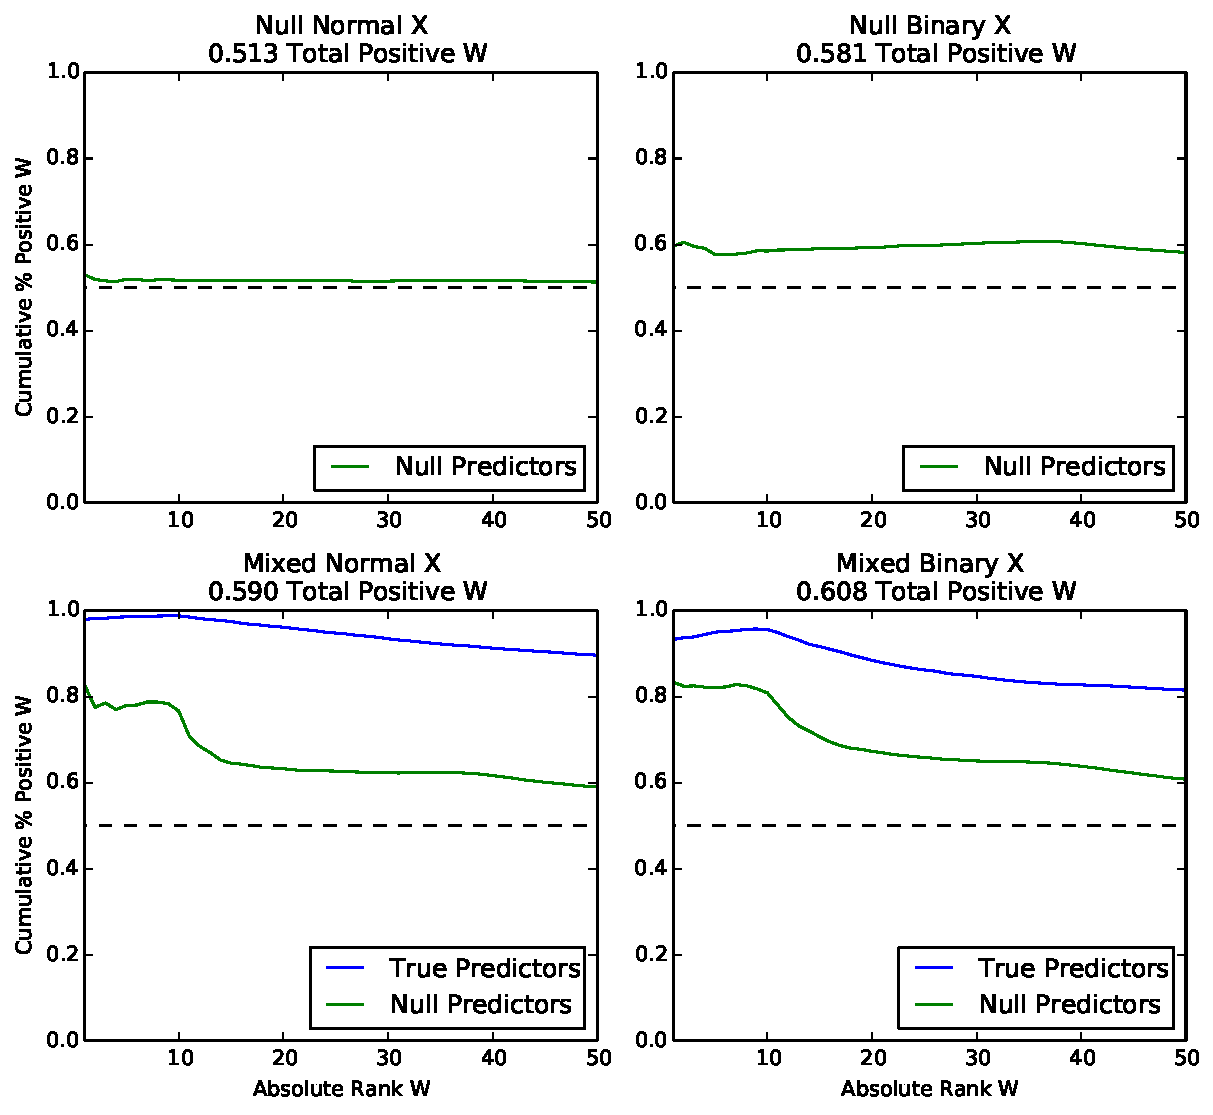
\includegraphics[width=14cm]{images/entryrate_original_logit}
    \end{center}
    \caption{\linespread{1}\selectfont{} The mean cumulative portion of $W$ statistic which are positive by absolute rank of the value. The mean is over 1000 simulations. On the left side, the features are drawn from a random standard normal distribution. On the right side, they are drawn as Bernoulli with probability $.25$ of being 1. The top has 50 null features, while the bottom has 10 features in the true model, and 40 null features.}
    \end{figure}
 
    \FloatBarrier


    To evaluate whether this made a difference in practice, I tested the method using original style knockoffs in logistic regression. The results can be seen in figure 1, which shows cumulatively, starting with the largest absolute value, what portion of the $W_j$ are positive. For the method to work, for the null predictors, this should be a consistent $50\%$, indicative of the desired symmetric distribution. This is particularly important for high values of $|W_j|$, which play the largest roll in selecting a threshold. In the top left corner, under the ``global null", where all features are null and normally distributed, we almost achieve this. There is just a small, but consistent, deviation from $50\%$. However, in the top right, when the predictors are binary but still all null, the originals enter first far more often, which will result in the FDR being too high. \par
    \begin{figure}[h]
        \begin{center}
            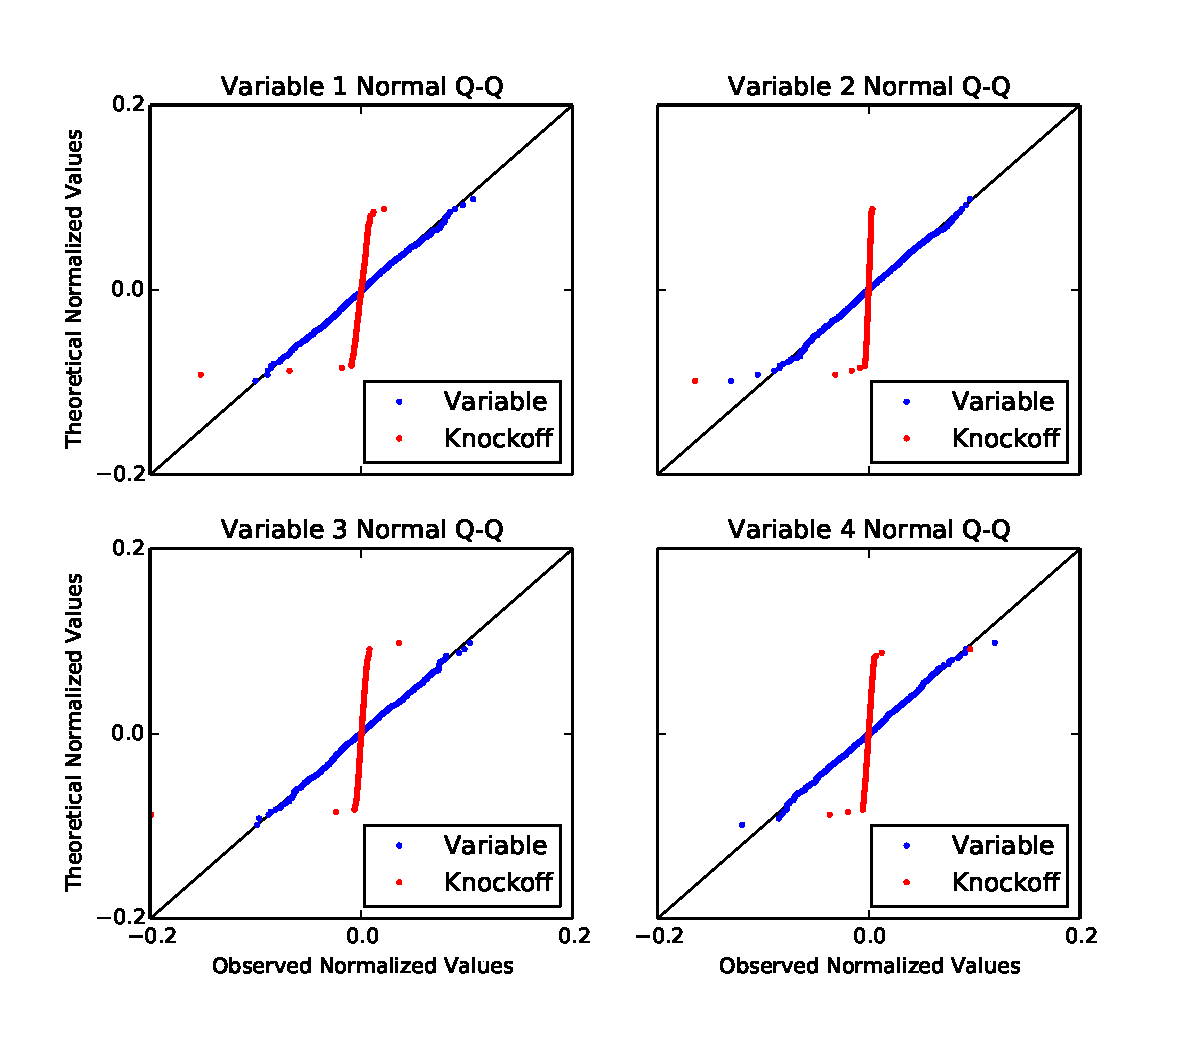
\includegraphics[width=14cm]{images/normalQQ}
            \caption{\linespread{1}\selectfont{}Normal Q-Q of original variables and knockoffs for simulation with $4$ variables and 1,000 observations}
        \end{center}
    \end{figure}

    This gets much worse when some true predictors are included in the model, as shown in the bottom row of the figure. For both normal and binary predictors, the originals come in first far more often in the beginning. This will completely ruin FDR control, since the portion of null predictors will be assumed far lower than it actually is. It is worth noting that the particular shape of the curve in the diagram, with the plateau for the null predictors through 10, is partially an artifact of there being 10 true signals. The mean through the first ten is the mean for null predictors that came in first out of both null and true predictors; since the largest ten $W_j$ will tend to be true predictors, the average over the null predictors represent the few extreme $W_j$ which managed to beat out some number of true predictors.  \par
    Upon examination, one issue seems to be that the original style knockoff features have a very different empirical distribution than the features they are imitating. This is obviously true with the binary features, but even with the normal features, the distributions differ substantially. In figure 2, the distribution of four features and their original style knockoff are plotted against a normal distribution in Q-Q plots. As you can see, the distributions differ substantially. This is suggestive of a solution; if the knockoff variables match the marginal distribution of the original features better, the result may be more suitable for FDR control in GLMs. \par
    \FloatBarrier

\section{Random Binary Knockoffs}
Coming up with knockoffs which would match the original features' marginal distributions better for arbitrary $X$ is daunting problem. Limiting ourselves to binary data, which is common in real world applications, presents a far more manageable case. However, solving for a binary $\tilde X$ which matches the correlation condition exactly or closely is an integer programing problem, which are generally NP-hard. Thus, instead, this section will develop methods of generating $\tilde X$ randomly such that the correlation condition holds in expectation. Mainly, $\tilde X\st X$ should be a random binary matrix such that
    \[ \E[X^T \tilde X \st X] = X^TX - \diag{\mathbf s} \quad \& \quad \E[\tilde X^T \tilde X \st X] = X^TX.\]



\subsection{Random Binary Vector Variables}
We can imagine each row of $X$ being an observation of a random binary vector variable $\mathbf x$. The full class of random binary vector variables on $\{0,1\}^p$ can be specified as multinomial on the $2^p$ elements of the set. However, it is generally impractical to specify or estimate all $2^p-1$ necessary parameters, so it is useful to pick a method to match the first two moments, as is desirable for knockoffs. These are the mean vector $\E(\mathbf x)=\mathbf{m}\in[0,1]^p$ and the cross-moment matrix $\E(\mathbf x\mathbf x^T)=M\in[0,1]^{p\times p}$. Obviously, $m_i = \p(x_i=1)$, $M_{ij} = \p(x_i=x_j=1)$, and $\mathbf m=\diag{M}$. For an arbitrary symmetric $M$ to be a valid cross-moment matrix for some random binary vector variable, the necessary and sufficient conditions are that $M-mm^T\succeq0$ and
    \[ \max\{0,m_i+m_j -1\} \leq M_{ij} \leq \min\{m_i,m_j\}\]
    for all $i\neq j$ \cite{2011arXiv1111.0576S}.

\subsection{Relaxed Correlation Condition}
As before with the original knockoffs, the first step of generating knockoffs is to decide on the target correlation structure for $X_{aug}$. For binary knockoffs, this is done by selecting the target covariance matrix $\Sigma_{aug}$. This is extremely similar, though not identical, to the method with the original knockoffs, where $X_{aug}^TX_{aug}$ after normalization was targeted. However, much the same method as before can be used. Let the vector of empirical means of the columns of $X$ be $\mathbf m = \frac{1}{n}X^T\mathbf 1$ and the empirical covariance matrix of $X$ be $\Sigma = \frac{1}{n}X^TX - \mathbf{m}\mathbf{m}^T$. Much as before with the original knockoffs, both the equi-correlated and SDP method can be used to select  $\mathbf s$  such that $\diag{\Sigma}-\mathbf s$ has small magnitude and 
        \[ \Sigma_{aug} = \left[\begin{array}{cc}  \Sigma & \Sigma - \diag{\mathbf s }\\ \Sigma - \diag{\mathbf s} & \Sigma \end{array}\right] \succeq 0. \]
    While with the original knockoffs, the result was small values for $X_i^T\tilde X_i$, now the result is low covariance between $X_i$ and $\tilde X_i$.\par
    Additionally though, the moment condition must hold for $\Sigma_{aug}$ to correspond to a proper random binary vector. If 
    \[\mathbf m_{aug} = \E\left(\mathbf x_{aug}\right) = \left[\begin{array}{c}\mathbf m \\ \mathbf m \end{array}\right] \]
    then the desired cross-moment matrix of the joint distribution is 
        \[ M_{aug} = \Sigma_{aug} + \mathbf m_{aug}\mathbf m_{aug}^T.\]
        As mentioned above, for this cross-moment matrix to correspond to an actual random binary vector, it must be the case  
        \[\max\{0,(m_{aug})_i + ( m_{aug})_j -1\} \leq (\Sigma_{aug})_{ij} +  (m_{aug})_i  (m_{aug})_j \leq \min\{( m_{aug})_i, ( m_{aug})_j\}. \]
    However, since $\Sigma$ and $\mathbf m$ are from an actual random binary vector, the entries of $\Sigma$ satisfy this property by default. Only off diagonal entries which have had $\mathbf s$ subtracted from them could possibly violate this condition. Furthermore, for these entries, the goal is to make $(\Sigma_{aug})_{ij}$ as close to $0$ as possible. Since the condition is always satisfied in a neighborhood of $(M_{aug})_{ij} = (m_{aug})_j(m_{aug})_i$, this implies that this method should normally be satisfied. This is the principle advantage of minimizing the $\textrm{cov}(x_i,\tilde x_i)$ rather than $\E[x_i\tilde x_i]$. For the SDP method though, the restriction can be built directly into the optimization problem. If $\sigma = \diag{\Sigma}^{\frac{1}{2}}$ is the vector of standard deviations, the updated problem is
            \begin{center}
                \begin{tabular}{r l}
                    minimize & $\|\mathbf 1-\diag{\sigma}^{-1}\mathbf s\|_1$ \\
                    subject to & $ 0 \preceq \diag{\mathbf s} \preceq 2\Sigma $ \\
                               & $ \max\{2m_i -1,0\} \leq \Sigma_{ii}-s_i + m_i^2 \leq m_i  \quad \forall i$
                \end{tabular} 
            \end{center} 
            the factor of $\diag{\sigma}^{-1}$ in the objective is to account for the $x_i$ not being normalized, as was the case with the original knockoffs. \par
            Given the $\Sigma_{aug}$ and corresponding $M_{aug}$, all that is needed is some process to generate $\tilde X$ that replicates the desired empirical cross moments. 


\subsection{Fitting via Quadratic Programing}
        The simplest way to do this is based on a probability matrix $P\in (0,1)^{n\times p}$, where each $X_{ij}$ is drawn independently as $X_{ij}\sim\textrm{Bernoulli}(P_{ij})$. Such a $P$ should satisfy 
            \begin{center}
                \begin{tabular}{r l}
                    minimize     & $\|X^TP-(M-\diag{\mathbf{s}})\|_{fro}^2 + \sum_{i\neq j}(P_i^T P_j - M_{ij})^2 $\\
                    subject to   & $ \mathbf 1^T P = \mathbf m $ \\
                                 & $0 \leq P \leq 1$
                \end{tabular} 
            \end{center}
            so that the cross-moments are as close as possible to $M_{aug}$. The first part of the objective corresponds to the deviation of $\E[X^T\tilde X]$ from $M-\diag{\mathbf{s}}$ and the second part to the deviation of $\E[\tilde X^T \tilde X]$ from $M$ excluding the diagonal values which are matched by $ \mathbf 1^T P = \mathbf m $. This problem can be stated as a quadratic program via the introduction of slack variables:
            \begin{center}
                \begin{tabular}{r l}
                    minimize     & $\|W\|_{fro}^2 + \|V\|_{fro}^2 $ \\
                    subject to   & $ -W \leq X^TP-(M-\diag{\mathbf{s}})\leq W $ \\
                                 & $ -V_{ij} \leq P_i^T P_j - M_{ij} \leq V_{ij} \quad \forall i\neq j$ \\
                                 & $ \mathbf 1^T P = \mathbf m $ \\
                                 & $0 \leq P \leq 1$
                \end{tabular} 
            \end{center}

            Though there are powerful tools and theory for solving quadratic programs, $n\times p$ would have to be fairly small for this optimization problem to be computationally reasonable in practice. Ideally, there would be a method to split up this problem into a series of smaller optimization problems which would yield the same solution. An optimist might hope that iterating through the columns of $P$, optimizing each to hit its desired cross-moments individually conditioned on the estimate of the rest of $P$, would achieve this. In practice, this does seem to yield reasonable results, and is far quicker than other methods for large $p$. In particular, the following method seems to work well:
    \begin{enumerate}
        \item Optimize initial $P_i$ such that $X_j^T P_i = M_{ij}$ if $i\neq j$ and $X_i^T P_i = M_{ii}-s_i$.   
            \begin{center}
                \begin{tabular}{r l}
                    minimize     & $ \left(\frac{1}{n}X_i^T P_i - ( M_{ii}-s_i)\right)^2 + \sum_{i\neq j}(\frac{1}{n}X_j^T P_i - M_{ij})^2$ \\
                    subject to   & $ \frac{1}{n}\mathbf 1^T P_i = M_{ii} $ \\
                                 & $0 \leq P_i \leq 1$
                \end{tabular} 
            \end{center}
        \item Draw initial $\tilde X_i$ as independent Bernoulli with probability $P_i$.
        \item Iterate through $1\leq i \leq p$, fitting new $P_i$ such that 
            \begin{center}
                \begin{tabular}{r l}
                    minimize     & $ \left(\frac{1}{n}X_i^T P_i - (M_{ij}-s_i)\right)^2 + \sum_{i\neq j}(\frac{1}{n}X_j^T P_i - M_{ij})^2 + \sum_{i\neq j}(\frac{1}{n}\tilde X_j^T P_i - M_{ij})^2$  \\
                    subject to   & $ \frac{1}{n}\mathbf 1^T P_i = M_{ii} $ \\
                                 & $0 \leq P_i \leq 1$
                \end{tabular} 
            \end{center}
            After each $P_i$ is fit, redraw $\tilde X_i$ as independent Bernoulli with probability $P_i$.
    \end{enumerate}
    Drawing the $\tilde X_i$ after each step, rather than just leaving the $P_i$, seems counter intuitive, but under experimentation, it seemed to provide better results. As well, though the third step may be repeated several times, in practice this didn't lead to improvement. 

\subsection{Fitting via Conditional Random Binary Vectors }
An alternate approach to generating $\tilde X$ that will satisfy the relaxed correlation condition is to find a random binary vector $\mathbf{x}_{aug}\in\{0,1\}^{2p}$ that has the desired cross-moments $M_{aug}$. Let $(\mathbf{x}_{aug})_1$ be the first $p$ entries of $\mathbf{x}_{aug}$ and $(\mathbf{x}_{aug})_2$ be the remainder. Then, for a row $\xi$ of $X$, the corresponding row $\tilde \xi$ of $\tilde X$ would be drawn from $(\mathbf{x}_{aug})_2\st (\mathbf{x}_{aug})_1=\xi$. This method necessitates a family of binary vectors which can match any cross-moment matrix and is easy to conditionally sample from.


\subsubsection{Gaussian Copula Family}
Since multivariate normal distributions are quite easy to sample from and are defined by their first two moments, an obvious choice is to use them to generate random binary vectors. This might be done by defining $x_i = \mathrm{sign}(z_i)$ for $\mathbf z\sim N_p(\mu,\Sigma)$, where $\mu$ and $\Sigma$ are chosen such that $\mathbf x$ has the correct cross-moments. However, this is only guaranteed to be feasible in the bivariate case. For higher dimensions, this method can generally only provide random binary vectors with approximately the right moments, and the quality of the approximation quickly degenerates as $p$ increases \cite{2011arXiv1111.0576S}. Therefore, we do not explore this direction further.

\subsubsection{$\mu$-Conditionals family}
There exists a more flexible family which will always work for arbitrary $M$ called $\mu$-conditionals \cite{2011arXiv1111.0576S}. The basic idea is that the entries of a binary vector variable $\mathbf x$ can be sampled sequentially as 
    \[ \p(x_{i}=1\st x_{1},...,x_{i-1}) = \mu\left(a_{ii}+\sum_{k=1}^{i-1}a_{ik}x_i\right) \]
    for some monotone function $\mu:\R\to(0,1)$. This is essentially a binomial family GLM for a link function $\mu$. If one takes all of the $a_{kj}$, they can form a lower triangular matrix $A$, and then the joint density can be expressed as 

    \[ \p(\mathbf x=\mathbf \xi) \propto \mu(\mathbf{\xi}^T A\mathbf \xi)\]

    If $\mu$ is chosen such that it is a bijection and differentiable, for any proper cross-moment matrix $M$, there is a corresponding $A$ such that $\E(\mathbf x \mathbf x^T \st A)=M$. The natural choice for $\mu$ is the logistic link function $L(x)=\frac{1}{1-e^{-x}}$, which yields the Ising model, the ``binary analogue of the multivariate normal distribution which is the maximum entropy distribution on $\R^p$ having a given covariance matrix." Additionally, it has the usual benefit that the coefficients are log odds ratios:
    \[a_{ij} = \log\left(\frac{\p(x_j=x_k=1)\p(x_j=x_k=0)}{\p(x_j=0,x_k=1)\p(x_j=1,x_k=0)}\right) \]
    when $i\neq j$. When $\mathbf x$ is generated from this model with $a_{ij}=0$, then $x_i$ and $x_j$ are conditionally independent.  \par

    There is no closed form to calculate the entries in $A$ if $p>1$, but they can be derived numerically two ways. The first of these, for when one is attempting to replicate the empirical cross-moments from a data matrix $X$, is to fit each row $a_{1i}$ to $a_{ii}$ by successive binomial family GLM regressions. The link function is the given function $\mu$, and $X_i$ is regressed on $X_{1} \ldots X_{i-1}$ using maximum likelihood. $a_{ji}$ for $i\neq j$ will then be the coefficient on $X_j$ in the model predicting $X_i$ while $a_{ii}$ is the intercept of the regression. \par
    Otherwise, if one is just working with a desired cross-moment matrix $M$, the successive rows of $A$ can be fit via Newton-Raphson \cite{2011arXiv1111.0576S}. This is performed successively on each row of $A$. If the first $i-1$ rows have been fit, then the upper left $(i-1)\times(i-1)$ sub matrix $A_{-i}$ of $A$ has already been filled. Next, $\mathbf a_i$, the first $i$ entries of the $i$th row of $A$ must be fit, while the rest of the row will be 0. This corresponds to $\mathbf m_i$, the first $i$ entries of the $i$th row of $M$. In other words, $\mathbf{m}_i = [\E(x_i x_j)]_{j=1}^{i}$. Finally, let us say that $\mathbf x_{-i}$ is the first $i-1$ entries of $\mathbf x$. $\mathbf a_i$ must satisfy 
            \begin{align*}
                \mathbf m_i &= \E\left(x_i \left[\begin{array}{c} \mathbf x_{-i} \\ x_i \end{array}\right]\right) \\
                 &= \E\left(\E\left(x_i \left[\begin{array}{c} \mathbf x_{-i} \\ x_i \end{array}\right]\;\bigg \vert\; \mathbf x_{-i}\right)\right)\\
                 &= \sum_{\xi_{-i} \in \{0,1\}^{i-1}} \p(\xi_{-i})\p(x_i=1\st \mathbf x_{-i}=\xi_{-i}) \left[\begin{array}{c} \xi_{-i} \\ 1 \end{array}\right] \\
            \end{align*}
            When $\mu$ is the logistic link function $L$, this is
            \[ \mathbf m_i = \sum_{\xi_{-i} \in \{0,1\}^{i-1}} \frac{1}{c}L\left(\mathbf \xi_{-i}^TA_{-i}\xi_{-i}\right) L\left(\mathbf{a}_i^T\left[\begin{array}{c} \mathbf \xi_{-i} \\ 1 \end{array}\right]\right)\left[\begin{array}{c} \xi_{-i} \\ 1 \end{array}\right] \]
            where $c$ is the appropriate normalizing constant. Let us define the quantity on the right in the last line as $f(\mathbf a_i)$. This equation $f(\mathbf a_i)=\mathbf{m}_i$ can be solved by successive Newton-Raphson iterations defined by 
            \[\mathbf a_i^{(k+1)} = \mathbf a_i^{(k)} - \left[J\left(\mathbf a_i^{(k)}\right) \right]^{-1}\left[f\left(\mathbf a_i^{(k)}\right)-\mathbf m_i\right] \]
            where $J$ is the Jacobian of $f$. To do so, the Jacobian matrix is calculated as 
        \[ J\left( \mathbf a_i\right) = \sum_{\xi_{-i} \in \{0,1\}^{i-1}} \frac{1}{c}L\left(\mathbf \xi_{-i}^TA_{-i}\xi_{-i}\right) L'\left(\mathbf{a}_i^T\left[\begin{array}{c} \mathbf \xi_{-i} \\ 1 \end{array}\right]\right)\left[\begin{array}{c} \xi_{-i} \\ 1 \end{array}\right]\left[\begin{array}{cc} \xi_{-i}^T & 1 \end{array}\right]. \]
            With $2^{i-1}$ possible values for $\mathbf x_{-i}$, this can quickly become computationally expensive. Instead, with K i.i.d. draws $\xi_{-i}^{(k)}\sim \mathbf x_{-i}$, the simulated values 
            \[f\left(\mathbf a_i\right) \approx \frac{1}{K}\sum_{k=1}^K L\left(\mathbf{a}_i^T\left[\begin{array}{c} \xi_{-i}^{(k)} \\ 1 \end{array}\right]\right)\left[\begin{array}{c} \xi_{-i}^{(k)} \\ 1 \end{array}\right] \]
            and
            \[J\left( \mathbf a_i\right) \approx \frac{1}{K}\sum_{k=1}^K L'\left(\mathbf{a}_i^T\left[\begin{array}{c} \xi_{-i}^{(k)} \\ 1 \end{array}\right]\right)\left[\begin{array}{c} \xi_{-i}^{(k)} \\ 1 \end{array}\right]\left[\begin{array}{cc} [\xi_{-i}^{(k)}]^T & 1 \end{array}\right] \]
            can be used. \par
            Though, in theory, $A$ should always exist, in practice limited accuracy may dictate that Newton-Raphson method won't converge. In the simulation method in particular, if $K$ is not large enough, the equations can be very difficult or impossible to solve. When the initial problem can't be solved, besides increasing the simulation size or numerical precision, one can instead solve the relaxed problem  $f(\mathbf a)=\mathbf m_i^*(\tau)$, where, for $\tau\in[0,1]$,
    \[\mathbf m_i^*(\tau) = (1-\tau)\mathbf m_i + \tau \left[ \begin{array}{cccc} 0 & \ldots & 0 & M_{ii} \end{array} \right]^T .\]
            When $\tau=0$, this yields the original problem, while when $\tau=1$, it is treats $x_i$ as independent of $\mathbf x_{-i}$. The latter will always have the solution
            \[\mathbf a_i = \left[ \begin{array}{cccc} 0 & \ldots & 0 & \log\left(\frac{M_{ii}}{1-M_{ii}}\right) \end{array} \right]^T.\]
            The hope is that for some $\tau$ close to $0$, convergence can be achieved, only causing a slight distortion from the desired cross-moments.

\subsubsection{Generating Binary Knockoffs from $\mu$-conditionals}
This suggests that an obvious choice for $\mathbf{x}_{aug}$ is to fit the $A$ for the Ising model which corresponds to $M_{aug}$ via the Newton-Raphson method. $A$ can then be used to generate a row $\tilde \xi$ of $\tilde X$ sequentially conditioned on the corresponding row $\xi$ of $X$ as $\tilde \xi_i \st \mathbf \xi,\tilde \xi_1,\ldots,\tilde \xi_{i-1}$. However, there are a few variations of this process which are preferable depending on the situation. 
        \begin{enumerate}
            \item If the whole $A$ matrix is being fit, then the upper half of the matrix, corresponding to $\mathbf x$, can be fit via the regression method, since they arise from real data $X$. This will tend to be quicker, since the calculation lends itself to parallel computing, and the data set will often be smaller than the space of all binary vectors or a simulation of that space. The second half of the matrix still must be fit via Newton-Raphson.
            \item One can avoid fitting the first half of the $A$ matrix entirely though by using the actual observed values in $X$ to simulate values $[\xi_1\ldots \xi_p]\sim \mathbf x_{aug}$ if performing the Newton-Raphson method. This can be done by either bootstrapping rows from $X$ or using some number of copies of $X$ exactly. The advantage of this is the saved computation and that $\mathbf{\tilde x}$ should be built to match the correlation condition more exactly. The downside is that, since these values won't be from the Ising model, the theoretical guarantee of a suitable $A$ may no longer hold. As well, if $n$ isn't big enough, the equations will quickly become difficult to solve, since the observed samples will provide a noisy and incomplete sample of the probability space.
            \item As $A$ is being fit, even the parts of $\mathbf x_{-i}$ corresponding to knockoffs need not be redrawn for each Newton-Raphson iteration or each successive $i$. To fit $\mathbf a_i$, the $\xi_{-i}^{(k)}$ will remain constant; then, once $\mathbf a_i$ has been fit, the $\xi_i^{(k)}$ need only be drawn once. This saves computation, and the multiplication
            \[ \left[\begin{array}{c} \xi_{-i}^{(k)} \\ 1 \end{array}\right]\left[\begin{array}{cc} [\xi_{-i}^{(k)}]^T & 1 \end{array}\right] \]
                needs only be partially recalculated for each Newton-Raphson iteration since the upper left portion, $\xi_{-i}^{(k)}[\xi_{-i}^{(k)}]^T$, won't change. This may result in slight deviations in any particular draw compounding into a more severe error over time.
            \item As $p$ grows large, and $K$ necessarily along with it, the cost of calculating the Jacobian matrix grows far quicker than the cost of calculating $f(\mathbf a)$. This is since it has $O(Kp^2)$ complexity compared to $O(Kp)$ complexity for $f(\mathbf a)$, which quickly becomes prohibitive. One might instead estimate the full Jacobian based on first differences, but in practice an even simpler method called Anderson mixing \cite{Fang07twoclasses}, which avoids additional computation of $f(\mathbf a)$, works well. Anderson mixing is one of several related quasi-Newtonian methods, which performs Newton-Raphson iteration $k$ with an approximation of the inverted inverted Jacobian labeled $G_k$. Thus, to solve for a variable $\mathbf z$ such that $f(\mathbf z)=\mathbf 0$, the best approximation for the root is updated as $\mathbf{z}_{k+1}=\mathbf{z}_k - G_k f(\mathbf{z}_k)$ at each iteration. \par
    Anderson mixing does this implicitly, with no extra recalculation of $f$, by approximating $f$ with the affine space spanning the previous $m$ evaluations of $f$. These values are $f(\mathbf z_{k})$ through $f(\mathbf z_{k-m+1})$. This is analogous to estimating the slope using a secant line, except in a high dimension space. The best approximation for $f(\mathbf z)=0$ in the affine space which spans them is defined by
    \[ \mathbf \alpha = \argmin_{\mathbf w:\, \sum_{i=1}^m w_i=1} \left\|\sum_{i=1}^m  w_i f(\mathbf z_{k-i+1}) \right\|_2 \]
    This leads to the updated approximation
    \[ \mathbf z_{k+1} = \sum_{i=1}^{m} \alpha_{i} \mathbf z_{k-i+1} \]
    $G_k$ doesn't need to be calculated here, and the quickest implementation finds $\alpha$ without calculating it. However, it's presence can be seen through an equivalent formulation. Let $\Delta \mathbf f_i = f(\mathbf z_k) - f(\mathbf z_{k-i})$, $\Delta \mathbf z_i = \mathbf z_k - \mathbf z_{k-i}$, 
    \[ \mathcal F = [\Delta \mathbf f_1 \ldots \Delta \mathbf f_{m-1}] \]
    and
    \[ \mathcal Z = [\Delta \mathbf z_1 \ldots \Delta \mathbf z_{m-1}] \]
    This means that $\mathbf\alpha$ has been replaced by $\mathbf\theta$ such that
    \[ \mathbf \theta \; = \;\argmin_{\mathbf w} \left\|f(\mathbf z_{k}) - \mathcal  F \mathbf w\right\|_2\; = \;(\mathcal F^T \mathcal F)^{-1}\mathcal F^Tf(\mathbf z_k) \]
    so 
    \[ \mathbf z_{k+1} \;= \;\mathbf z_{k} - \mathcal Z \mathbf \theta\; = \; \mathbf z_{k} - \mathcal Z(\mathcal F^T \mathcal F)^{-1}\mathcal F^T f(\mathbf z_k) \]
    Which yields the approximated inverse Jacobian $G_k= \mathcal Z(\mathcal F^T \mathcal F)^{-1}\mathcal F^T$
        \end{enumerate}
        In practice, it seemed that combining the first, third, and fourth of these variations leads to the most successful technique. However, should $n$ be large enough to provide a good approximation of the probability space, the second variation also saves a lot of time.\footnote{An implementation of this method in python can be found on my github: \url{https://github.com/ajmaurer/Chicago-Course-Work/blob/master/masters_paper/knockoffGLM.py}}

\section{Binary Knockoff Performance}
    While the theory for original knockoffs and random binary variable generation suggests at how the binary knockoffs should behave, seeing their actual performance still provides invaluable insight to their uses and limitations. There are three major areas in which this is useful: how well do the binary knockoffs' empirical cross-moment matrices converge to their expectation, how well is FDR controlled for linear regression, and how well, if at all, is FDR controlled for other GLMs? \par
    To answer each of these questions, I performed a number of different simulations of the random binary knockoffs. In each one, the rows of $X$ were drawn from the Ising model with a randomly generated $A$ matrix for the specified $p$. Where $z_{ij}\sim N(0,.2)$, $A_{ij}=z_{ij}$ if $i\neq j$, and $A_{ii}=z_{ii}-1$ otherwise. This leads to mild correlation among the columns of $X$. Then, for $i\in S$, $\beta_i\sim N(0,1)$, being otherwise set to $0$. For each observation for the linear regressions, $y\sim N(\mathbf{x}^T\beta,1)$, while for the logistic regressions, $y\sim \textrm{Bernoulli}(L(\mathbf{x}^T\beta))$. Given $X$, $\tilde X$ was generated based by the $\mu$-conditional method.

\subsection{Convergence to Theoretical cross-moments} 
    \FloatBarrier
        In a certain sense, the question of the convergence of the binary knockoffs' empirical cross-moments is the least interesting of the given questions. Assuming the Ising model coefficient $A$ or the probability matrix $P$ was successfully fit, the cross-moment matrices' will converge to their expectation in probability for increasingly large values of $n$. However, especially with the limited numerical accuracy available to fit $A$ or $P$, the rate at which this convergence occurs and the size of the deviation is an issue of paramount importance. As is seen in Figure 3, this convergence occurs at similar rates irrespective of $p$, with fairly meaningful deviation until $n$ has reached a few thousand.
    \begin{figure}[h]
        \begin{center}
            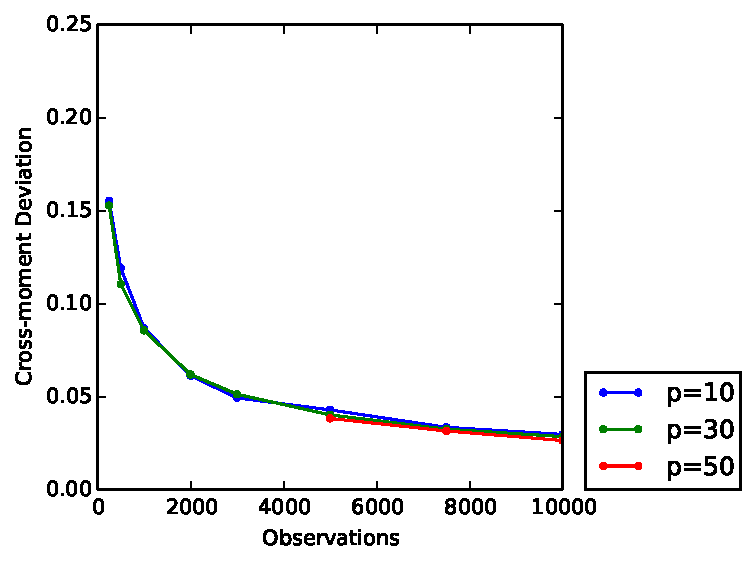
\includegraphics[width=9cm]{images/sigma_fit}
    \end{center}
    \caption{\linespread{1}\selectfont{}Measures how much far the empirical cross-moment matrix $\frac{1}{n}X_{aug}^TX_{aug}$ is from the desired cross moment matrix $M_{aug}$ for random binary knockoffs for various $n$ and $p$, averaged over $50$ simulations. Where $W = \Sigma - \diag{\mathbf s} + \mathbf m \mathbf m^T$ is the top quadrant of $M_{aug}$, deviation is calculated as $(\|X^T\tilde X - W\|_{fro} + \|\tilde X^T \tilde X - M\|_{fro})/(\|W\|_{fro}+\|M\|_{fro})$, where $\| \cdot \|_{fro}$ is the Frobenius norm.}  
    \end{figure}


    \FloatBarrier
\subsection{Performance in Linear Regression} 
    \FloatBarrier
    When the knockoff filter is used in linear regression, we see that the original knockoffs are still superior to the binary knockoffs. As figure 4 shows, while they both fail to control the FDR when there are only a few true predictors\footnote{This issue is addressed in the original paper; a slightly more conservative filter called knockoff+ avoids this problem}, the original knockoffs properly control FDR when there is a larger number of valid predictors. That it does so rather conservatively is a reflection of the relatively low number of total features compared to the sparsity. On the other hand, though mirroring the trend with the original knockoffs, the binary knockoffs fail to exactly control FDR at level $q=.2$. They select too many variables, which gives higher power at the expense of proper FDR control. As figure 5 shows, both methods make related, but non-identical, variable selections. \par
    
    \begin{figure}[h]
        \begin{center}
        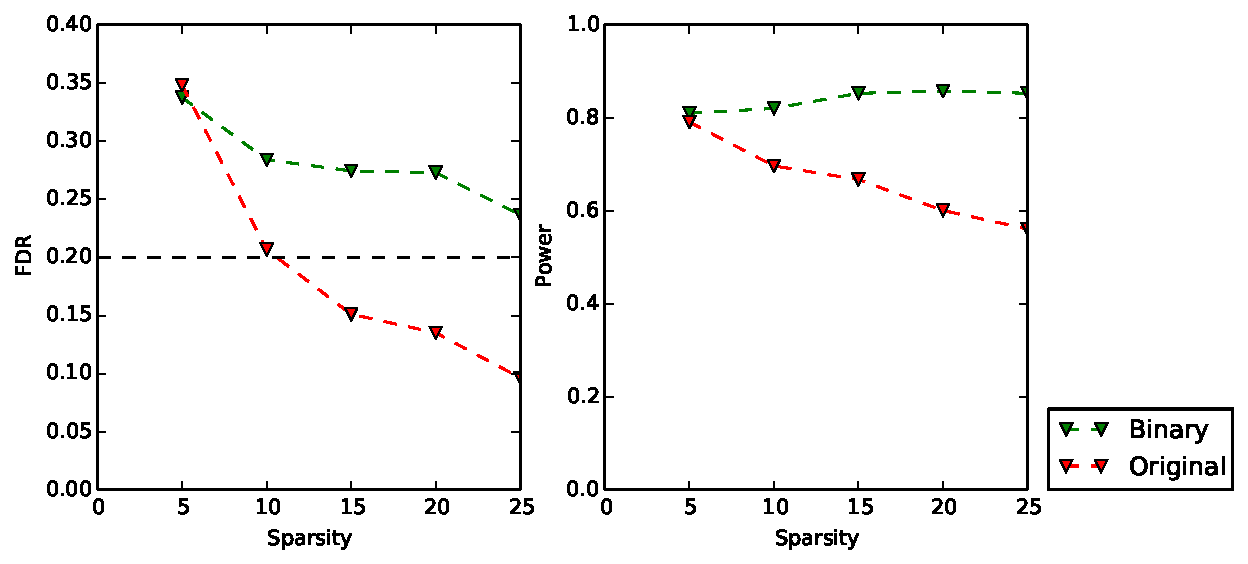
\includegraphics[width=14cm]{images/lasso_FDR_power_50}
    \end{center}
    \caption{\linespread{1}\selectfont{}The mean FDR and power of binary and original knockoffs. Taken over $200$ simulations of linear regression on $n=1000$, $p=50$, and targeting FDR $q=.2$ for varying levels of sparsity.}  
    \end{figure}

    \begin{figure}[h]
        \begin{center}
        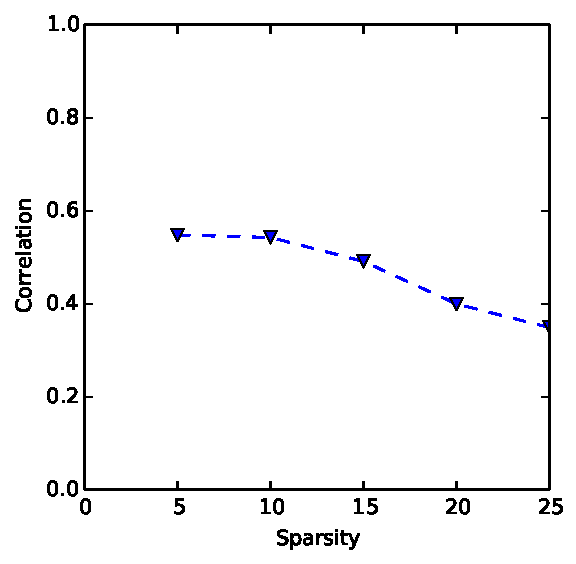
\includegraphics[width=7cm]{images/lasso_corr_50}
    \end{center}
    \caption{\linespread{1}\selectfont{}Mean correlation between $z_i=I_{\hat S}(i)$ for binary knockoffs and for original knockoffs. Taken over $200$ simulations of linear regression on $n=1000$, $p=50$, and targeting FDR $q=.2$ for varying levels of sparsity.}  
    \end{figure}
    This is disappointing, but shouldn't be surprising. The binary knockoffs only replicate the correlation structure of the original features in expectation, rather than exactly. Thus, for any given value $n$, the empirical correlation of the combined design matrix $X_{aug}$ won't exactly be $\Sigma_{aug}$, and the method won't work perfectly. However, even here, the actual FDR is only somewhat higher than the desired $.2$, and for larger values of $n$, the empirical correlation will get closer to $\Sigma_{aug}$, and the FDR will be controlled better.

    \FloatBarrier
\subsection{Performance in Logistic Regression} 
    \FloatBarrier
    In logistic regression, the binary knockoffs do seem to provide an improvement over the original knockoffs, as can be seen in figure 6. Though neither control FDR exactly at $.2$, using binary knockoffs result both in higher power and lower FDR. As well, while the original knockoffs do considerably worse in logistic regression than in linear regression, the binary knockoffs perform only a little worse, having similar FDR and somewhat lower power. This suggests that much of the excess FDR is due the deviation from the desired correlation matrix. It should be noted though that this simulation is very favorable towards the binary knockoffs; the design matrix $X$ is generated from the Ising model, which is also the model used to generate the binary knockoffs. It is quite likely that for $X$ generated with significant high order interactions, the binary knockoffs wouldn't perform as well, though still likely better than the original knockoffs. 
    \begin{figure}[h]
        \begin{center}
        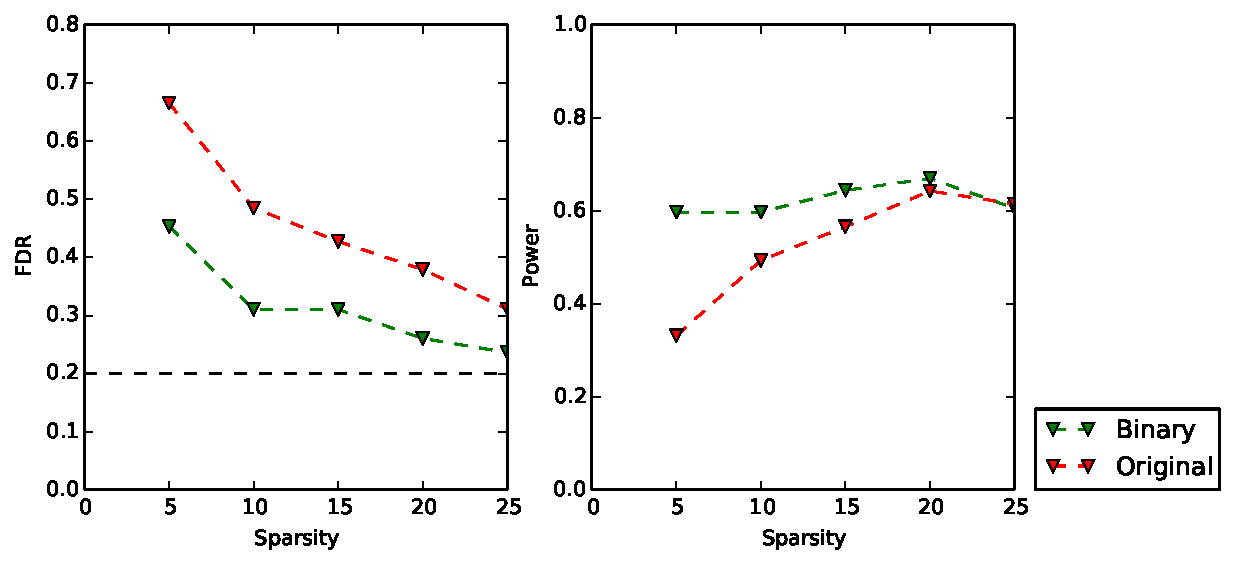
\includegraphics[width=14cm]{images/logit_FDR_power_50}
    \end{center}
    \caption{\linespread{1}\selectfont{}The mean FDR and power of binary and original knockoffs. Taken over $200$ simulations of logistic regression on $n=1000$, $p=50$, and targeting FDR $q=.2$ for varying levels of sparsity.}  
    \end{figure}

    \begin{figure}[h]
        \begin{center}
        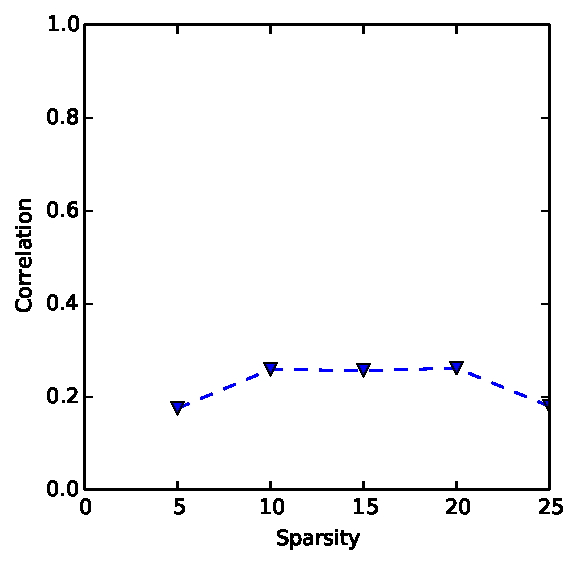
\includegraphics[width=7cm]{images/logit_corr_50}
    \end{center}
    \caption{\linespread{1}\selectfont{}Mean correlation between $z_i=I_{\hat S}(i)$ for binary knockoffs and for original knockoffs. Taken over $200$ simulations of logistic regression on $n=1000$, $p=50$, and targeting FDR $q=.2$ for varying levels of sparsity.}  
    \end{figure}

    \FloatBarrier

\section{Discussion}
    This paper has developed a method, along with several variations, of creating random knockoffs for binary data. These knockoffs serve as a replacement in the knockoff filter for the original style knockoffs; they serve the same purpose, but rather than meet the correlation condition exactly, they meet it in expectation. Since they are generated randomly so that they satisfy the correlation condition in expectation only, we see that in simulations they only provide approximate FDR control for linear regression. However, since they imitate the marginal distribution of the original $X_i$, they provide much better FDR control in logistic regression than the original style knockoff. \par
    As a practical tool for statistical inference, they are still a work in progress. They do seem to provide approximate FDR control in logistic regression. However, there are no theoretical guarantees for this to be true, and the quality of FDR control for LASSO depends on how far the realized cross-moment matrix deviates from the desired $M_{aug}$. In cases where $n$ is large, this should only be a small issue, but for smaller $n$, FDR control fails in a meaningful way. As well, computational issues make binary knockoffs hard to generate for large $p$; as $p$ increases, the Ising model to generate the knockoffs gets rapidly more computationally intensive to fit, as do the methods based on quadratic programs. This leaves the method, as currently developed, only suitable for relatively high values of $n$ and low values of $p$. \par
    However, this method, with the real possibility of extending the knockoff filter to GLMs, offers an interesting development if these issues can be resolved. For the issue with the deviation from the desired cross-moment matrix, a solution would likely take the form of an ensemble method. Rather than fit the $A$ and $P$ matrix to generate one $\tilde X$, several $\tilde X$ might be generated and used to make variable selections $S_m$. A finally variable selection $S$ could be made based on theses, perhaps only selecting the variables selected by the majority of the $S_m$. This, or some other sort of average across multiple realizations of $\tilde X$, could likely be used to dampen the effect of variance in the generation of $\tilde X$ so as to make binary knockoffs more reliable for both LASSO and other GLMs. \par
    The computational issues will likely be more difficult to deal with. As $p$ increases, a larger and larger matrix $A$ must be fit for the Ising model as well as a larger $P$ for the quadratic program. For the Ising model, the simulation size $K$ must similarly grow to provide accurate estimates of the probability space. This causes an explosion in computation time. Some of this can likely be mitigated by improvements in implementation, and the most time intensive issue, calculating $f(\mathbf a)$, can be easily parallelized. Still, a less computationally intensive method to derive either $A$ or $P$ is necessary to make $p$ in the hundreds or thousands feasible. A method based on optimizing each column of $P$ individually is thus appealing. So far, only approximate solutions have resulted from this method. However, in similar situations, other methods, such as the EM algorithm, have been developed which have strong guarantees for global optimization using such piecewise optimization. If a similar development could be made here, or merely a method that hits the desired cross-moments more closely in practice, the result would be far more useful tool. \par
    The final area of concern is how binary knockoffs will perform when the $X$ matrix is not fit well by the Ising model due to significant high order interactions. Hopefully, having matched the first and second moments of $X$, binary knockoffs will continue to provide reasonable FDR control. One avenue to ensure this would be to explicitly model these higher order interactions. We might introduce higher order moments into the fitting of $\mu$-conditionals. For instance, $A$ could be a three dimensional matrix whose entry $a_{ijk}$ would be added to the linear predictor when $x_i=x_j=x_k=1$. Just as the $\mu$-conditionals are based on a regression of $X_i$ on $X_{1:i-1}$ with no interactions, this would be akin to adding two-way interactions. This can be used to replicate arbitrary binary vectors to an arbitrary desired level of precision. However, this has big limitations. For one, adding additional levels of interactions will make the computation much more difficult very quickly. As well, as far as generating knockoffs, it will become more and more difficult to reduce the correlation between $x_i$ and $\tilde x_i$ as higher order interactions are insisted on. Nonetheless, this may be an avenue for further investigation. \par
   
\nocite{*}
\printbibliography[heading=bibintoc]
\end{document}
